\documentclass[10pt]{article}

\usepackage{fancyhdr}
\usepackage{extramarks}
\usepackage{amsmath}
\usepackage{amsthm}
\usepackage{amsfonts}
\usepackage{tikz}
\usepackage{ragged2e}
\usetikzlibrary{automata,positioning}
\usepackage{setspace}
\usepackage{etoolbox}
\usepackage{enumitem}
\usepackage{hyperref}
\hypersetup{colorlinks=true,allcolors=blue}
\usepackage{hypcap}
\usepackage{graphicx}    %for figure environment.
\usepackage{calc}
\usepackage{ifthen}
\usepackage{tikz}
\usepackage{longtable}
\usepackage{lipsum}
\usepackage{verbatim}
\usepackage{enumitem}
\setlist[enumerate]{itemsep=0mm}
\setlist[itemize]{itemsep=0mm}
\usepackage{pstricks-add}
\usepackage{pstricks}
\usepackage{rotating}
\usepackage[]{algorithm2e}
\usepackage{pdfpages}


\makeatletter
\pretocmd{\@sect}{\singlespacing}{}{}
\pretocmd{\@ssect}{\singlespacing}{}{}
\apptocmd{\@sect}{\singlespacing}{}{}
\apptocmd{\@ssect}{\singlespacing}{}{}
\makeatother

%
% Basic Document Settings
%
\newcommand{\ts}{\textsuperscript}

%\begin{comment}
\topmargin=-0.45in
\evensidemargin=0in
\oddsidemargin=0in
\textwidth=6.5in
\textheight=9.0in
\headsep=0.25in
%\end{comment}

\linespread{1.1}

\pagestyle{fancy}
\lhead{\hmwkAuthorName}
\chead{\textbf{\hmwkClass : \hmwkTitle}}
\rhead{\hmwkAuthorNumber}
\lfoot{\lastxmark}
\cfoot{\thepage}

\renewcommand\headrulewidth{0.4pt}
\renewcommand\footrulewidth{0.4pt}

\setlength\parindent{0pt}

%
% Create Problem Sections
%


\setcounter{secnumdepth}{0}
\newcounter{partCounter}
\newcounter{homeworkProblemCounter}
\setcounter{homeworkProblemCounter}{1}
\nobreak\extramarks{Problem \arabic{homeworkProblemCounter}}{}\nobreak{}

%
% Homework Problem Environment
%
% This environment takes an optional argument. When given, it will adjust the
% problem counter. This is useful for when the problems given for your
% assignment aren't sequential. See the last 3 problems of this template for an
% example.
%


%
% Homework Details
%   - Title
%   - Due date
%   - Class
%   - Section/Time
%   - Instructor
%   - Author
%

\newcommand{\hmwkTitle}{Assignment 3\ \ }
\newcommand{\hmwkDueDate}{Sunday, December 3\ts{rd}, 2017}
\newcommand{\hmwkClass}{CSC411}
\newcommand{\hmwkClassTime}{Section A}
\newcommand{\hmwkClassInstructor}{Steven Chuang}
\newcommand{\hmwkClassTeachingAssistant}{Natalia Mykhaylova}
\newcommand{\hmwkAuthorName}{Gokul K. Kaushik}
\newcommand{\hmwkAuthorNumber}{999878191}
\newcommand{\schoolmate}{\textsc{School-Mate }}

\newcommand\Tstrut{\rule{0pt}{2.6ex}}       % "top" strut
\newcommand\Bstrut{\rule[-0.9ex]{0pt}{0pt}} % "bottom" strut
\newcommand{\TBstrut}{\Tstrut\Bstrut} % top&bottom struts
%
% Title Page
%

\title{
    \vspace{2in}
    \textmd{\textbf{\hmwkClass:\ \hmwkTitle}}\\
    \vspace{0.1in}\small{Due\ on\ \hmwkDueDate}\\
    \vspace{3in}
    \vspace{0.1in}\large{Student Name: \textbf{\hmwkAuthorName} } \\
    \vspace{0.1in}\large{Student Number: \textbf{\hmwkAuthorNumber} } \\
}

%\author{\textbf{\hmwkAuthorName}}
%\textbf{\hmwkAuthorNumber\}
\date{}

\renewcommand{\part}[1]{\textbf{\large Part \Alph{partCounter}}\stepcounter{partCounter}\\}

%
% Various Helper Commands
%

% Useful for algorithms
\newcommand{\alg}[1]{\textsc{\bfseries \footnotesize #1}}

% For derivatives
\newcommand{\deriv}[1]{\frac{\mathrm{d}}{\mathrm{d}x} (#1)}

% For partial derivatives
\newcommand{\pderiv}[2]{\frac{\partial}{\partial #1} (#2)}

% Integral dx
\newcommand{\dx}{\mathrm{d}x}

% Alias for the Solution section header
\newcommand{\solution}{\textbf{\large Solution}}

% Probability commands: Expectation, Variance, Covariance, Bias
\newcommand{\E}{\mathrm{E}}
\newcommand{\Var}{\mathrm{Var}}
\newcommand{\Cov}{\mathrm{Cov}}
\newcommand{\Bias}{\mathrm{Bias}}
\renewcommand*\contentsname{Table of Contents}

\begin{document}
\maketitle
\pagebreak

\begin{center} \tableofcontents \end{center}
\pagebreak

\clearpage
\setcounter{page}{1}

\section{1 - 20 Newsgroup Predictions}
\section{2 - Training SVM with SGD}
\subsection{2.1 - SGD with Momentum}
\subsection{2.2 -Training SVM}
\subsection{2.3 - Apply 4-vs-9 Digits on MNIST}
\subsubsection{2.3.1 - Training Loss}
\subsubsection{2.3.2 - Test Loss}
\subsubsection{2.3.3 - Classification Accuracy on the Training Set}
\subsubsection{2.3.4 - Classification Accruacy on the Test Set}
\subsubsection{2.3.5 - Plot \textbf{$w$} as a 28 $\times $ 28 image }


\section{3 - Kernels}
\subsection{3.1 - Positive Semi definite and Quadratic Form}
\subsection{3.2 - Kernel Properties}
\subsubsection{3.2.1 - Prove Property}
\subsubsection{3.2.2 - Prove Property}
\subsubsection{3.2.3 - Prove Property}
\subsubsection{3.2.4 - Prove Property}



\pagebreak


\end{document}

$

\section{1 - Class Conditional Gaussians}
This page has been left blank. The math solutions are handwritten on the next page onwards.

%\includepdf[pages=-,pagecommand={},width=\textwidth]{math.pdf}

\section{2 - Handwritten Digit Classification}
\subsection{0 - Loading the data and Plotting the Feature Means}

The means (from 700 samples per digit) for each feature (64 features in total for an 8-by-8 pixel image) for 10 digits (digit 0 to digit 9) are plotted below: 

\begin{center}
%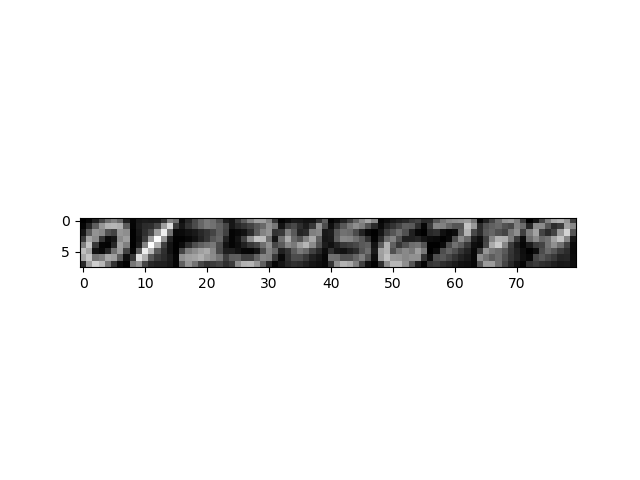
\includegraphics[scale=1]{averages.png}
\end{center}


\subsection{1 -  K-NN Classifier}
\subsubsection{2.1.1 Train and Test Classification Accuracy for K=1 and K=15}

Training Data Classification Accuracy for K=1: 1.0
\\
Training Data Classification Accuracy for K=15: 0.961
\\
Test Data Classification Accuracy for K=1: 0.96875
\\
Test Data Classification Accuracy for K=15: 0.959


\subsubsection{2.1.2 Tie Breaker Method}

There are cases in K-Nearest Neighbours where there isn't one most frequent neighbours (there might be two neighbours that occur equally frequently). Therefore, in such cases a tie breaking decision needs to be made. I have chosen to reduce the number of nearest neighbours by one - \textbf{effectively removing the last neighbour and repeating the check until a decision can be made}.
\\ \\
This method was chosen because: 
\begin{enumerate}
\item The tie remains until the \textit{most distant} neighbour from one of the most frequent neighbours is removed. This rewards the neighbour with the closest value in such cases.
\item This decision making method is intuitive to understand and easy to implement.
\end{enumerate}

\subsubsection{2.1.3 Optimal K}

\textbf{The optimal K from applying 10-folds on the data set is K=3.}
\\ \\
Training Data Classification Accuracy for K=3 on 10-folds: 0.9865
\\
Test Data Classification Accuracy for K=3 on 10-folds: 0.9697


\subsection{2 -  Conditional Gaussian Classifier Training}

\subsubsection{2.2.0 Plot of the Diagonal Elements of the Covariance Matrix}

\begin{center}
%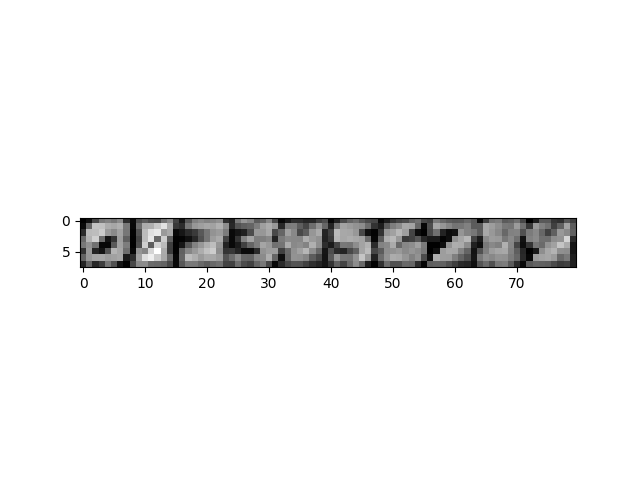
\includegraphics[scale=1]{covariances.png}
\end{center}

\subsubsection{2.2.1 Average Conditional (Log) Likelihoods}

The average conditional (log) likelihoods were compute for the train set and the test set are:
\begin{center}
\textbf{Train Data Set: } -0.124624436669
\\
\textbf{Test Data Set: } -0.196673203255
\end{center}

\subsubsection{2.2.3 Accuracy for the Most Likely Posterior Class}

For the most likely posterior class, the training and test set accuracies are: 
\begin{center}
\textbf{Train Data Set: } 0.9814
\\
\textbf{Test Data Set: } 0.9727
\end{center}


\subsection{3 -   Naive Bayes Classifier Training}

\subsubsection{2.3.3 Plot of Eta}

\begin{center}
%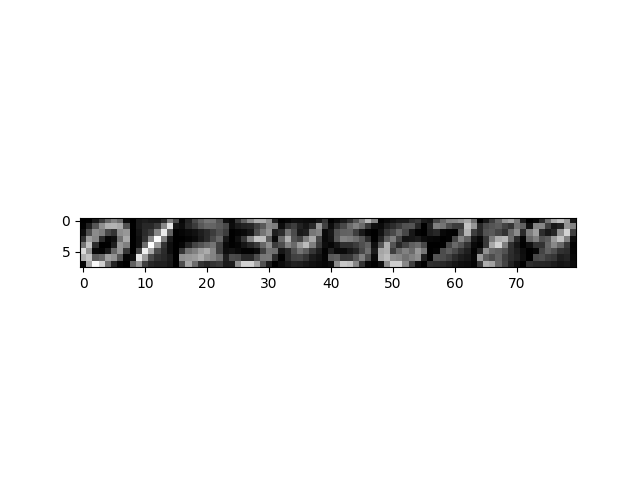
\includegraphics[scale=1]{q2_3_1.png}
\end{center}

\subsubsection{2.3.4 Plot of Generated Binarized Data (Using a Binomial Disribution)}
\begin{center}
%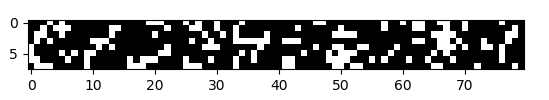
\includegraphics[scale=1]{q2_3_1_binomial.png}
\end{center}


\subsubsection{2.3.5 Average Conditional (Log) Likelihoods}

The average conditional (log) likelihoods were compute for the train set and the test set are:
\begin{center}
\textbf{Train Data Set: } -0.9437538618
\\
\textbf{Test Data Set: } -0.987270433725
\end{center}

\subsubsection{2.3.6 Accuracy for the Most Likely Posterior Class}

For the most likely posterior class, the training and test set accuracies are: 
\begin{center}
\textbf{Train Data Set: } 0.7741
\\
\textbf{Test Data Set: } 0.7642
\end{center}



\subsection{4 -  Model Comparison}

The models performed from (best to worst): 
\begin{enumerate}
\item Conditional Gaussian Classifier
\item K-Nearest Neighbours
\item Naive Bayes Classifier
\end{enumerate}

Conditional Gaussian Classifier obtained a test accuracy of 97\% followed by the KNNs (for K=3) at 96\% and then the Naive Bayes Classifier at 0.76\%.
\\ \\
The superior performance of the conditional Gaussian Classifier over the Naive Bayes Classifier would make sense as Naive Bayes assumes more assumptions (in terms of independence among features, which did not exist).
\\ \\
The independence among features does not exist because if a pixel was shaded black, the surrounding pixels would be probably black also. From black to white (in pixels), there is a gradual change. This change is hi-lighted by the covariance matrix. If there was a relationship between certain features, it would be greater than 0. 
\\ \\
The K-NNs surprisingly performed worse as the number of neighbours increased. One would have assumed that increasing the size of K would smooth the decision plane boundaries. One reason could be that the number of samples per digit (700) was too small to see an improvement in performance. However, the fact that after K=3 shows that after 3, it becomes hyper-sensitive towards neighbour boundaries. This is one explanation.


